\subsection{Towards Automatic Learning of Procedures from Web Instructional Videos}

\subsubsection{Overview}

\par Luowei Zhou \textit{et al}, in their 2017 paper titled \textit{Towards Automatic Learning of Procedures from Web Instructional Videos} \cite{zhou2017automatic}, introduced the problem of \textit{procedure segmentation}. The goal was to divide the long and unconstrained instructional videos into category-independent procedure segments using visual features. They present \textit{ProcNets} for generating this proposals. They also introduce the dataset of 2000 cooking videos - YouCook2.


\subsubsection{Datasets}
\begin{itemize}
\item YouCook2
\end{itemize}

\subsubsection{Performance}
\par Zhou \textit{et al} compared their model with video summarization LSTM and segment CNN for proposals using Jaccard and mean IoU. ProcNets performed better in terms of both the metrics. They report state-of-the-art performance with F1 score of 33.4\% in proposal localization.


\subsubsection{Methodology}

\par ProcNets consists of three components:
\begin{enumerate}
	\item Feature encoding
	\item Segment proposal module for candidate proposals
	\item Sequential prediction for final proposals
\end{enumerate}

\begin{figure}[h]
	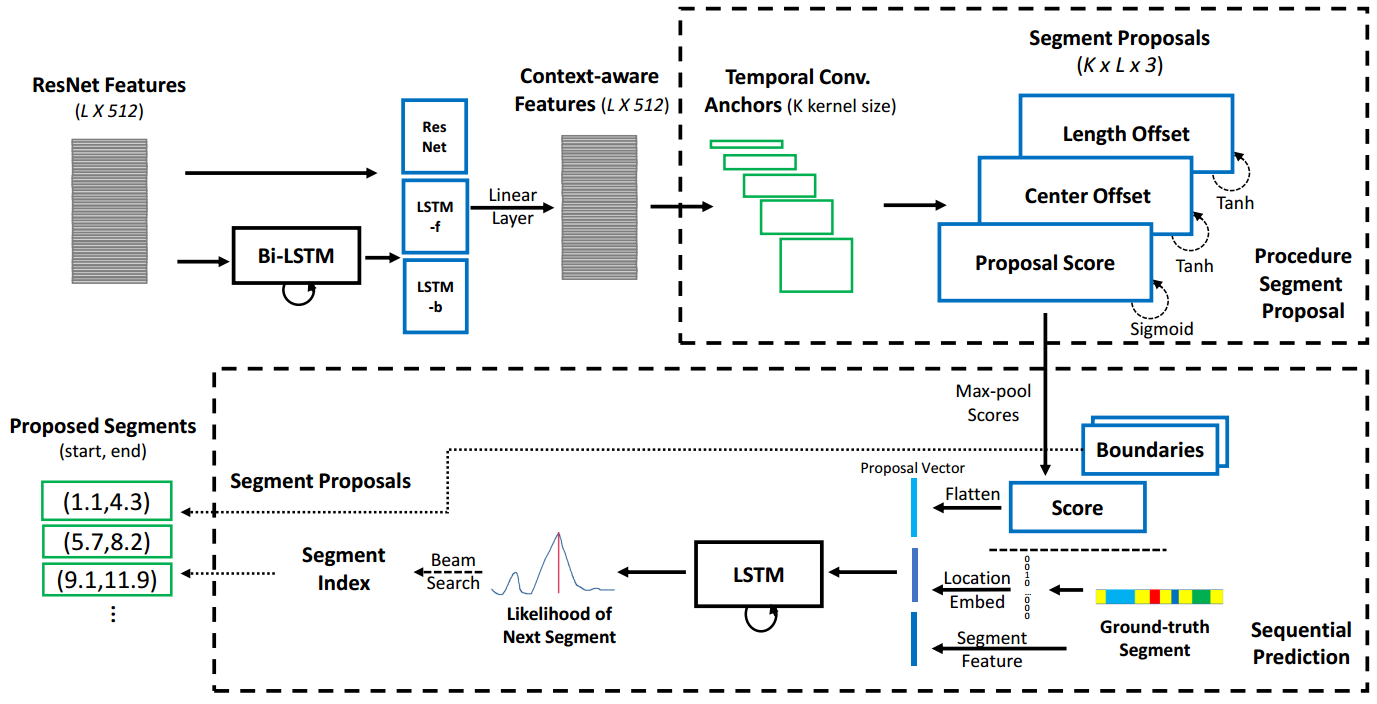
\includegraphics[width=\linewidth]{assets/img/zhou2017automatic-architecture.png}
	\caption{ProcNets introduced by Zhou \textit{et al} (taken from \cite{zhou2017automatic})}
\end{figure}

\paragraph{ProcNets}
\begin{enumerate}
	\item Sampling video into 500 frames and calculating feature encoding for each frame using ResNet \cite{he2015deep} and Bi-LSTM.
	\item Segment proposal module takes in encoded features and output proposal candidates {score, center offset, length offset} using anchor-offset mechanism inspired by Faster R-CNN \cite{ren2016faster}.
	\item Sequential prediction module uses LSTM for selecting final proposals.
	\item The input to LSTM is as follows:
	\begin{enumerate}
		\item S: max-pooled proposal score vector
		\item $B_t-1$: location embedding of previous segment
		\item $C_t-1$: mean-pooled ResNet features of previous segment 
	\end{enumerate}
\end{enumerate}


\subsubsection{Conclusion}

\par Zhou \textit{et al} presented ProcNets for the task of proposal generation. The work concentrated on procedural videos with events that barely overlap and have long range dependencies among segments. They showed how the network learn temporal dependency among segments and give poor results on the permuted version of videos.